\documentclass[conference]{IEEEtran}

\sloppy

%\pdfpagewidth=8.5in
%\pdfpageheight=11in


\usepackage{graphicx}
\usepackage{epstopdf}
\usepackage{subfigure}
\usepackage{wrapfig}
\usepackage{caption}
%\usepackage{subcaption}
%\usepackage{subfig}
\usepackage{amsmath}
\usepackage{xspace}
\usepackage{authblk}
\usepackage{url}

\graphicspath{ {../fig/} }

% enable/disable margin comments
\newif\ifcomments
%\commentsfalse
\commentstrue

%\pagestyle{headings}

\begin{document}

\title{FLUX: A Next-Generation Resource Management Framework for Large HPC Centers}
\author{Dong H. Ahn, Jim Garlick, Mark Grondona, Don Lipari, Becky Springmeyer, 
        Martin Schulz\\        \{ahn1,garlick,grondona1,lipari1,springme,schulzm\}@llnl.gov}
\affil{Lawrence Livermore National Laboratory, Computation Directorate, 
        Livermore, CA 94550}

\date{}
\maketitle


\newcommand{\flux}{Flux\xspace}
\newcommand{\zMQ}{\O{}MQ}


\begin{abstract}
Resource management (RM) software is crucial to HPC
for efficient application execution. %on a set of resources.
%
However, growing numbers and types of compute resources
and a greater interplay among various resources 
(e.g., between compute clusters and a shared I/O cluster) 
%across the entire HPC center can render even 
can render even
the best-in-breed RM software increasingly ineffective.
HPC centers are at a junction where they require
a new paradigm for resource management
to meet the challenges of extreme scalability,
resource diversity, and increasing complexity of job and resource
constraints such as power budgeting.
Our response to this critical need is \flux, an RM software
framework that can solve the key RM challenges
in a simple, extensible, distributed, and autonomous fashion.
Its design targets a computing facility as one common pool
of diverse sets of resources to provide
efficient and informed scheduling decisions and flexible accommodation
of site-wide constraints.

Further, \flux\ employs a framework approach to facilitate 
the seamless integration of system monitoring and administration,
lightweight virtualization, and  parallel programming and tools
run-time systems.
In this paper, we discuss our vision for \flux, identify key design challenges
and concepts, and report our progress prototyping
key components.
We report preliminary results that show our run-time prototype
provides requisite properties such as high scalability
and easy integration, as well as interoperability among essential
run-time software programs. %elements such as MPI, run-time tools and middleware.
\end{abstract}

%\keywords{{resource management, communication framework, run-time,
%key value store, scalable process management services.}}
\section{Introduction}

Scalable Resource and Job Management Software (RJMS) is critical
for High Performance Computing (HPC).
It is the centerpiece that enables efficient
execution of HPC applications while providing
the compute center with the means
to maximize the utilization of its diverse  
 computing resources~\cite{GeorgiouThesis}.
However, current state-of-the-art RJMS systems 
are becoming increasingly
ineffective in dealing with the growing diversity and size 
of resources fielded in HPC centers today. Large-scale 
resources are no longer limited to  
%As numbers and types of compute resources
%continue to grow, the key management challenges 
%traditionally associated with only 
a few extremely large individual machines 
like Sequoia (LLNL)~\cite{sequoia}, % or Titan (ORNL)~\cite{titan}, 
%quickly 
but are becoming commonplace through all computing resources sited at a center, including
commodity Linux clusters.
A modern RJMS must provide management services 
to all of the resources at the center,
while maintaining
scalability, low noise, fault tolerance, and enforcing global constraints.
%and heterogeneity management delivered 
%within increasingly stricter power bounds.

In addition, greater difficulties in code development
on larger systems impose increasingly challenging
%requirements on the RJMS, 
requirements on 
debugging, tuning, testing, and verification
%of applications have become too difficult and 
%time-consuming for end-users
%Next-generation code development environments
%require the RJMS to provide effective mechanisms
%to ease this user burden with features that support 
%the reproducible results of program execution,
as well as new techniques for 
%provide 
accurate correlations between user-level errors
and system-level events.
These tools
require adequate RJMS support~\cite{STAT,SPINDLE,PRUNER,SCR,launchmon}
for launching of daemons, allocation of analysis resources, or the ability
for secure third-party access to running jobs.
%,
%and facilitate integration and development 
%of a rich set of scalable tools.
Unless the RJMS can effectively
address these requirements, HPC users 
may suffer significant productivity losses
across the full application development life-cycle. 

The traditional resource and job management paradigm
for large HPC centers organizes the resources sited
at a center in a static and flat hierarchy. Typically, it 
runs an RJMS instance such as SLURM~\cite{Jette02slurm}
to manage and schedule an individual cluster,
and those instances are often connected
together by {\em separate} job management software, 
like MOAB~\cite{MOAB}, PBS Pro~\cite{PSBPro}, and LSF~\cite{LSF}.
While simple, the increasing interplay 
between various classes of compute resources 
across the center renders this paradigm often
inflexible and ineffective. 
For example, this paradigm cannot effectively
schedule applications that utilize site-wide shared 
resources such as file systems. 
Without scheduling file I/O-intensive jobs 
to both compute resources and file systems, 
overlapping I/O bursts coming from only a handful of 
unrelated jobs can disrupt the entire center~\cite{SCR,SPINDLE}. 
In addition, with such an inflexible and shallow hierarchy, 
dynamically imposing complex 
resource constraints at various levels at the center
is becoming increasingly intractable. 
%Avoiding any significant site-wide bottleneck
%requires the RJMS to schedule the job to all dependent
%resources that often span the boundaries 
%of a single cluster.

To address these challenges, we need 
%In this paper, we argue for 
a new management paradigm that is capable of scalably managing 
all of the resources (e.g., compute, storage, and visualization)
at a center together {\bf under one common RJMS framework},
(co-)scheduling jobs to these various types of resources, and 
dynamically enforcing global and local resource constraints. 
% that can
%effectively address the resource and job management 
%challenges that large HPC centers are increasingly facing.
%We argue that the new paradigm 
%must increase its purview 
%to manage resources across the entire center under
%one common RJMS framework, and 
%be able to 
The only way to achieve this with scalability in terms of the total number 
of resources as well as jobs is that the RJMS system must
%Further it mustWe argue that the new paradigm must 
facilitate management and scheduler parallelism~\cite{Omega,Mesos}
and further provide this parallelism through hierarchical, multilevel 
management and scheduling schemes with support for arbitrary numbers of levels.
The latter also requires capabilities for customization or specialization (in terms
of policy, access control, etc) at any level of this dynamic hierarchy 
based on user requests.
%, and 
%be capable of specializing each level.

In this paper, we present \flux, a new open-source RJMS framework that implements 
this new paradigm. We will describe
its design and run-time architecture and show how it will be capable of providing
the necessary RJMS capabilities for next-generation systems and centers. To
demonstrate its feasibility, we have prototyped and evaluated two of its core run-time components:
%
%We have implemented key aspects
%of the \flux 
%
%
%It will be a long journey to fully implement this new paradigm. 
%But we have made a few significant steps to embody the paradigm:
%we started to develop an open-source RJMS framework, \flux,
%and to explore its run-time core components.
%Thus, this paper also presents our early explorations
%of two core run-time elements: 
the communication framework termed the Comms Message Broker (CMB)
and Key Value Store (KVS) to hold \flux state.
%
%
%workload run-time services for efficient, interoperable
%launching and organizing of the distributed processes --- 
CMB and KVS together represent a novel back-bone overlay network for \flux,
which can replace all the redundant and independent
daemon infrastructures that currently exist in a typical cluster.

This paper makes the following contributions:
\begin{itemize}
\item{We describe, based on experience in one of the world's largest HPC centers, the emerging resource and job management challenges that demand a new paradigm;}
\item{We present the design and run-time architecture of \flux, a novel RJMS system that embodies this new paradigm;}
\item{We evaluate two of the core run-time components of \flux to demonstrate the feasibility of our approach.}
\end{itemize}

The results of our performance evaluation 
and performance models show that both KVS and CMB provide 
strong and predictable scaling properties and provide a scalable foundation 
for the \flux architecture.
%Further, our case study on integrating various key run-time software software
%programs indicate that \flux's run-time elements 
%provide these programs with 
%easy integration and interoperability.
%These results continue to guide our design choices
%as we progressively realize our vision. 


\section{A New Management Paradigm for HPC}
\label{label:paradigm}
HPC centers typically provide a wide range of 
platforms on which scientific applications perform
computations.
The RJMS system is responsible for efficiently delivering 
compute cycles of these platforms
to multiple users submitting jobs to run their applications. 
To enable this, the RJMS matches users' job request with the available 
resources and provides efficient functions 
for building, submitting, launching and executing, 
and monitoring jobs~\cite{GeorgiouThesis}. 
Typically, an HPC center runs an RJMS instance~\cite{Jette02slurm} 
to manage an individual system (e.g., cluster) and 
grid software often ties these instances together. 

However, several growing trends present major challenges 
to the current management paradigm. 
First, systems sited at one center are growing larger 
and types of resources are becoming increasingly diverse~\cite{GeorgiouThesis}. 
%The RJMS must now provide  
%extreme scalability, low
%noise, fault tolerance, and heterogeneity management
%to most of the resources sited across the entire center. 
Second, interplays between 
various classes of resources
(e.g., between compute clusters and a global file system)
are becoming more complicated and disruptive~\cite{SCR,SPINDLE}. 
Third, resource constraints are also becoming increasingly
complex in a multidimensional and hierarchical fashion~\cite{power-overprovision}
(e.g., dynamic power capping at the level of systems, compute racks, and/or nodes).
Further, the need for code development tools and their requirements on tool launching and job access
impose challenging requirements on the RJMS~\cite{STAT,SPINDLE,PRUNER,SCR,launchmon}.
Finally, the workloads themselves are becoming 
diverse, dynamic, and large, and are moving away from individual monolithic jobs. Instead
ensembles of jobs, e.g., for Uncertainty Quantification 
%DONG: We need a refernece to use Scalebriging Application
or Scalebriding Applications, are becoming increasingly commonplace.

To address the issues effectively,
large HPC centers demand a new resource and job management paradigm.
The new paradigm must increase its purview
to manage resources across the entire center
{\bf under one common RJMS framework}. Only this allows
%This would allow the 
centers to (co-)schedule jobs 
to various types of resources and to
provide much richer provenance on jobs (e.g., correlation between
a user-level error and other system activities). The new paradigm, however,
creates a series of challenges a new RJMS must overcome:

%It is important to note that all of these must 
%be enabled by one common RJMS framework. 
%The current paradigm of loosely coupling different software 
%(i.e., grid software with cluster-wide RJMS instances) 
%leads to a loss of important system knowledge
%needed for effective resource and job management and scheduling. 
%Different software employ distinct resource and
%job representations and key data are often lost in translation.
%Also, the single common framework can offer 
%common run-time commonents as a backbone of
%supporting hierarchical management of resources and jobs
%in a highly scalable, fault-tolerant, secure and customizable
%manner.

%We realize that embodying the new paradigm is non-trivial, as
%the following characterizes the challenges it must address.

\noindent{\em Challenge 1: Multidimensional Scaling --- } 
The new paradigm requires that the RJMS can impose
complex, multidimensional resource bounds at any scale, 
from the center-wide level, down to the level of individual processes,
and enable the most efficient execution and
scheduling of workloads within these bounds.
This imposes unprecedented scale challenges
in multiple dimensions,
%We generally characterize this challenge 
%as the {\em multidimensional scale} challenge. The challenges
% include
supporting extreme scalability, addressing noise as concurrency
increases, and managing a drastically increased amount of
run-time information that must be monitored, traced, and stored.
The new paradigm must efficiently handle increased scale in
numbers of resources as well as jobs and other dimensions 
of RJMS data.

\noindent{\em Challenge 2: Diverse workloads --- }
HPC applications are known to have disparate performance 
limiting factors. This requires
the new paradigm to have a rich resource model, including
the 
%This includes a 
representation for diverse
types of resources such as file systems, networks, visualization
hardware, and heterogeneous compute engines.
With a richer resource model, the RJMS will be capable of imposing
complex, multidimensional resource bounds, as opposed to the
simplistic traditional resource model that is fundamentally based on a
flat list of nodes, allowing it to 
%With the ability to model sophisticated resource relationships,
%the new paradigm will be able to schedule and
allocate resources tailored to the disparate limiting
factors of HPC applications.  

\noindent{\em Challenge 3: Dynamic Workloads --- }
Resource allocations
must be elastic, i.e., resource allocations must be able to grow and shrink
dynamically. This is necessary to support HPC applications with different
phases with disparate performance-limiting factors.
Different resource types have different
elastic properties 
(e.g., power is a much more elastic resource than compute nodes)
restricting decision points and allocation granularity.
%HPC applications and their programming models are
%becoming increasingly dynamic with different multi-resource requirements
%at different phases. 
One consequence of this its that the RJMS must 
support multiple levels of elasticity~\cite{Convergence} 
as a function of dynamically changing performance limiters
as well as their limiting resource types---e.g., 
rigid vs. moldable vs. malleable scheduling 
against different workload and resource types.

\noindent{\em Challenge 4: Productivity --- }
The new paradigm must address increasing complexities
in code development and system administration by facilitating
the creation of more effective diagnostic and analysis tools.
For example, it must provide basic, scalable monitoring and communication
primitives at the job level that can be leveraged by tools.
It will encourage a richer, stronger tool ecosystem.
% where
%these basic but non-trivial capabilities need not be recreated
%from scratch in every tool, reducing development costs.
Better tools will lead to higher productivity for all
stakeholders, including end users.
%We characterize this design challenge as the {\em productivity challenge}.

\noindent{\em System Challenges --- }
In addition to these main requirements that come from the user side
of the RJMS, we also face internal challenges that need to be hidden
from the user. 
%We have considered additional challenges. 
For example, in a global model,
the risk of higher downtime costs arises. 
%in a more global model.
If the RJMS is inadequately designed, a downtime could negatively
impact the availability of a large portion of the center's
resources. Thus, it must be tolerant of hardware and software
faults and failures with no single point of failure and 
also support live software upgrades. 
Other challenges include security, integration risk, 
and backwards compatibility. 
%will be addressed in our future work.

%

To address these challenges, %Undoubtedly, such a new paradigm will face unprecedented scaling challenges.
%in job scheduling. a RJMS 
%Thus, it 
the new RJMS must facilitate scheduler
parallelism~\cite{Omega,Mesos} through hierarchical,
multilevel resource management and job scheduling.
In this scheme, higher-level schedulers
should allow a site to impose site-wide policies, contracts,
and constraints while lower-level schedulers should allow
efficient use of any subsets of resources in accordance with
workload types.
The new paradigm must dynamically support arbitrary levels in
such a resource and job hierarchy with an ability to impose
different constraints at each level.



\subsection{Conceptual Software Design}
We describe some of our primary conceptual models
that will embody this new paradigm while addressing
the multitude of design challenges described above.
These models form the basis for the software design
of FLUX.

\vspace{1ex}
\noindent{\em Unified Job Model:} Traditionally, a job is
simply defined to be a resource allocation, a concept
too weak to support the new paradigm. Rather, we unify
the traditional job notion with the notion of a resource
manager instance---an independent set of resource
manager services. The RM instance must be delegated
the main responsibility of managing the resources allocated
to the job. Then, the unified job model becomes
the foundation on which to build a hierarchical, 
resource-management scheme to address the multidimensional
scale challenge. In addition, an RM instance can
implement compatibility mode with a particular
traditional paradigm only over its own allocation, 
providing a straightforward path to address
the backward compatibility challenge.

\vspace{1ex}
\noindent{\em Job Hierarchy Model:} To scale the new paradigm
in the scaling limit of the entire computing facility, 
we must avoid a centralized approach: the new paradigm 
requires a hierarchical management scheme with a well-balanced, 
multilevel delegation structure. For this purpose, 
we use a tree-based job hierarchy model that has 
many proven advantages for extreme scalability. 
In this model, a job is only required to manage 
its children jobs, which would be only a small fraction 
of the total number of jobs that are run across 
the entire computing facility. Further, several guiding 
principles throughout the job hierarchy strike 
a balance between the management responsibility 
of a parent job and delegation and empowerment 
of a child job:

\begin{enumerate}
\item{Parent bounding rule: the parent job grants 
and confines the resource allocation of all of its children.}

\item{Child empowerment rule: within the bound set 
by the parent, the child job is delegated the ownership 
of the allocation and becomes solely responsible 
for most efficient uses of the resources.}

\item{Parental consent rule: the child job must ask 
its parent job when it wants to grow or shrink the resource 
allocation, and it is up to the parent to grant the request.}
\end{enumerate}

In general, these rules enforce the first principle 
of the new paradigm: imposing highly complex resource bounds 
to guarantee the highest operational efficiency 
at any level across the computing facility, while enabling 
most efficient execution and scheduling of the workloads 
within these bounds. 

At the same time, this model is the most fundamental 
design concept, which forms the basis to address 
many of the design challenges including 
the {\em multidimensional scale}, {\em dynamic workload}, 
{\em power}, and {\em scheduling challenges}.

\vspace{1ex}
\noindent{\em Generalized Resource Model:} In the traditional 
paradigm, compute resources are modeled primarily 
as a collection of compute nodes, a simplistic perspective 
ill-suited for the new paradigm. Today's applications 
are diverse with disparate limiting performance factors 
beyond floating point computation. 

Further, computing centers are increasingly concerned 
about managing new resource types such as power 
and shared persistent storage. The generalized resource 
model is our concept to represent various resource types 
and their relationships that can impact how well applications 
perform and the computing facility operates. 
Our generalized resource model also includes a unified 
resource specification and description language. 
Speaking the same resource description language 
for request specification provides transparency and 
fine-grained expressibility. Our generalized resource 
model addresses not only the {\em diverse workload} 
and {\em power challenges}, but the {\em scheduling challenge}.

More specifically, the unified language approach 
allows users to express their resource requests 
more flexibly, e.g., using ranges or boolean 
expressions instead of hard amounts to allow requests 
to be fulfilled from several equivalent resource types. 
This makes the scheduling granularity 
of jobs finer and more malleable.

\vspace{1ex}
\noindent{\em Resource Allocation Elasticity Model:} As our 
applications and their programming models are becoming 
increasingly dynamic, the new paradigm must support 
an elasticity model where an existing resource allocation 
can grow and shrink, depending on the current needs 
of applications and/or the computing facility. 

We support the elasticity model within our job hierarchy 
framework above: a child job sends a grow or shrink request 
to its parent, which can go up the job hierarchy 
until all requisite constraints are known for this request. 
Also, combining this with the generalized resource model, 
the elasticity can be expressed for any resource including 
power consumption. Our elasticity model not only addresses 
the {\em dynamic workload} and {\em power} challenges, but also 
{\em scheduling challenge}. When a significant schedule stall 
is created with no small jobs to backfill, some of the 
currently running jobs can grow into these stalled 
resources and possibly complete sooner.

\vspace{1ex}
\noindent{\em Common Scalable Persistent Communication Infrastructure Model:} 
Our scalability strategy with respect to a large number 
of compute nodes is to provide a common scalable communication 
framework within each job. When a job is created, a secure, scalable 
overlay network with common communication service is established 
across its allocated nodes. Except for the root-level job, 
the existing communication session of the parent job assists 
the child job with rapid creation of its own session. 

A communication session is only aware of its parent 
and child and passes the limited set of control information 
through this communication channel. Thus, this model 
enables highly scalable communication within a job, while 
limiting communications between jobs, addressing 
both the {\em multidimensional scale} and {\em security challenges}. 

Further, this backbone per-job communication network 
supports many well-known bootstrap interfaces 
for distributed programs including many MPI implementations 
as well as run-time tools, and thus in part addresses 
the {\em productivity challenges}.

\vspace{1ex}
\noindent{\em Self-Hosting Model:} We use a self-hosting model 
to instantiate a new RM instance: the parent is capable 
of launching a standalone copy of itself as a child job, 
but possibly with different plugins. This makes it easier 
for developers or a quality assurance team to test 
new RM versions, helping addressing the 
{\em higher downtime costs challenge}. Further, self-hosting 
with new and experimental plugins encourages 
experimentation and facilitates research activities 
within a production instance, addressing 
the {\em productivity challenges}, too

\vspace{1ex}
\noindent{\em Lightweight Virtualization Model:} The lightweight 
virtualization model is our response to the 
{\em higher downtime costs}, {\em separation-of-concerns} 
and {\em security challenges}. Full-fledged virtualization 
techniques like Xen and Kernel-based Virtual Machine (KVM) 
have many advantages for these design challenges, but 
that approach has proven to be ineffective for HPC 
due in large part its high overhead~\cite{VirtHPC}. 
Instead, our virtualization strategy exploits OS-enforced
resource management and isolation mechanisms 
to launch applications in containers with virtually 
no impact on performance~\cite{ContainerVirt}. Within a container, 
private file system namespaces allow the system 
and applications to have divergent file system views, 
and to access file systems with different constraints.


\section{Preliminary Approach to \flux\ Run-time System}


It is a serious undertaking 
to design the production version of a new 
RM framework that can realize our proposed conceptual models.
Thus, \flux\ team has charted its course through a series of steps
meant to inform our design process. 
We began with a functional design that includes an
internal review with various stakeholders including 
developers at the operating systems level
as well as run-time and applications level.
Then, our initial research thrust was the run-time system of \flux.

%Then, this notion provided us with a concise 
%mechanism by which we can relate groups of processes
%to underlying resources (e.g., containing certain processes 
%to a set of resesources) as well as relate groups
%one another (e.g., synchronizing tool processes to 
%MPI processes). 
%
For our run-time, we have developed prototypes of our communication framework 
called Communication Message Broker (CMB) 
and a scalable key value store (KVS) service.
They comprise essential scalable building blocks of our run-time system, 
and we have begun to build various run-time services and also 
to port user-level run-time software programs to them.
Further, we introduced the notion of lightweight 
job (LWJ) as a new way to organize distributed or parallel processes.
Using this notion, a wide range of run-time software
programs such as parallel programming models,
tools and middleware can all leverage our run-time services 
to build on the strength of one another 

\ifcomments
\marginpar{\tiny BS: Do you want to now make a case for why KVS is going
to be an important building block?  Or just launch into the next
two sections on CMB and V'S?}
\marginpar{\tiny DA: I think I made a case. Let me know if not}
\fi

\subsection{Communication Message Broker}

A communication framework supports our hierarchical job model
by establishing a {\em comms session} to contain each \flux instance
and provide a foundation for the distributed components upon which
\flux is built.
As this framework must follow our common communication infrastructure
model, it enables secure, scalable communication
within a comms session, limits communication between sessions,
and allows new comms sessions to be created, resized, destroyed,
and monitored by existing ones in a parent-child relationship.
The framework is persistent for the life of a \flux job and is 
shared among \flux services, tools, and application run-times.

\begin{figure}
\centering
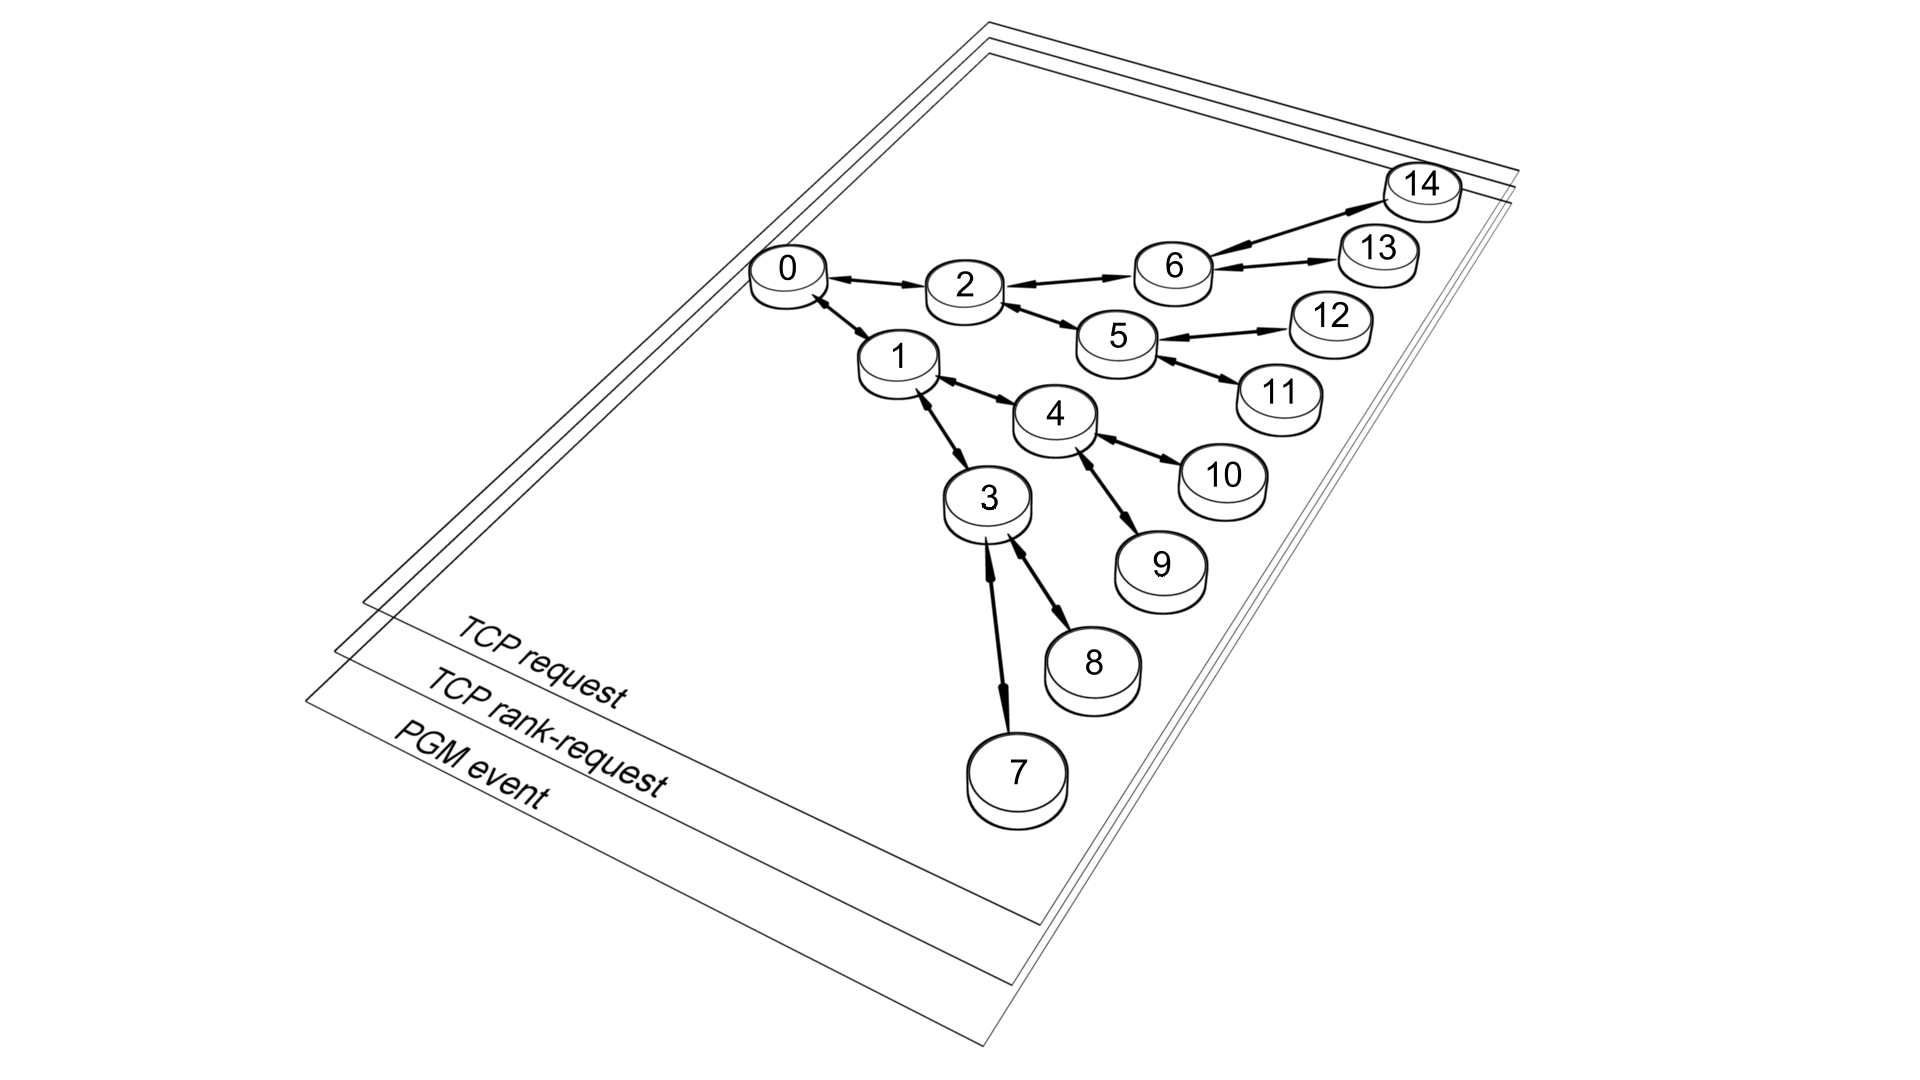
\includegraphics[trim=5.0cm 8.0cm 5.0cm 8.0cm,scale=0.12]{B_Tree_4Layer_BW2}
\vspace{.8cm}
\caption{A comms session} 
\vspace{-.5cm}
\label{fig:commswireup}
\end{figure}

We have built a prototype of the framework using the \zMQ~\cite{ZMQGuide}
%which we can launch within a
%Slurm~\cite{Jette02slurm} job.
messaging library, which provides the ability to pass messages securely
over multiple transports, including TCP, UNIX domain IPC, shared memory, and
Pragmatic General Multicast (PGM)~\cite{rfc3208}.
%\zMQ\ can be used to build applications or custom message brokers.
Its socket-like API abstracts common messaging patterns such as
{\em request-reply}, {\em publish-subscribe},
and {\em push-pull}.

Our prototype consists of a distributed Comms Message Broker (CMB)
daemon that runs on each node of a comms session, interconnected using
three persistent overlay network planes:
a PGM {\em publish-subscribe} bus for events and synchronization heartbeats;
a TCP {\em request-response} tree for scalable RPCs, barriers, and reductions; and
%similar to those enabled by MRNet~\cite{mrnet}; and
a secondary TCP {\em request-response} overlay with configurable topology
for rank-addressed RPCs.

%consists of daemons interconnected using
%three persistent overlay network planes:
%a TCP {\em dealer-router} tree for upstream RPCs and reductions,
%a TCP {\em dealer-router} tree for downstream RPCs, and
%a PGM {\em publish-subscribe} bus for events.
%Although a binary tree is pictured, the RPC planes can be launched in
%any tree shape for testing or to tune performance.
%%Flat, degenerate, {\em k}-ary for several values of {\em k}, and
%binomial have been tested.
%}

The comms session wire-up is depicted in Figure~\ref{fig:commswireup}.
Each message plane implements reliable, in-order message delivery, and
can self-heal when interior nodes fail.
Although a binary RPC/reduction tree is pictured, the tree shape is
configurable.
A design for comprehensive fault tolerance, including root node failure,
is a near-term project activity.

The CMB allows us to experiment with loosely coupled distributed services
that share this message routing framework. The various service components
of \flux have
been implemented as {\em comms modules}, plugins which are loaded into the
CMB address space and pass messages over shared memory.
Comms modules currently exist for the components listed
in Table~\ref{tab:cmbmod}.
Each embodies an active topic for study and experimentation.
% by the \flux\ team.

In addition to comms modules, external programs communicate with the CMB
over a UNIX domain socket.  A {\tt flux} utility wraps command line access
to about two dozen modular \flux\ sub-commands, and a custom PMI~\cite{PMI2}
library allows MPI run-times to access the \flux\ KVS and collective barrier
modules over this transport.

\begin{table}
\centering
\vspace{-.5cm}
% implement basic building blocks for \flux\ and
%potentially other applications.  These are the plugins we have prototyped
%thus far, representing a wide range of design maturity.  Each embodies an
%active topic for study and experimentation by the \flux\ team.}
\begin{tabular}{|l|p{7cm}|}\hline
\textbf{Plugin} & \textbf{Description} \\
\hline
hb & A periodic heartbeat event multicast across the comms
	session synchronizes background activity to reduce scheduling jitter.\\
\hline
live & Each tree node receives heartbeat-synchronized {\em hello}
	messages from its children.  After a configurable number of missed
	messages, a liveness event is issued for a dead child.\\
\hline
log & Log messages are reduced and filtered before being placed in
	a log file at the session root.  A circular debug buffer
	provides log context in response to a fault event.\\
\hline
mon & Lua scripts stored in the KVS activate heartbeat-synchronized sampling.
	Samples are reduced and stored in the KVS.\\
\hline
group & \flux groups define and manage collection of processes that can
	participate in collective operations.\\  
\hline
barrier & Collective barriers provide synchronization across \flux groups. \\
\hline
kvs & A distributed key-value store provides a scalable multi-purpose data store
	for \flux and other tools operating within the comms session.\\
\hline
wrexec & Remote processes can be launched in bulk, monitored,
	receive signals, and have standard I/O captured in the KVS.\\
\hline
resrc & Resources are enumerated in the KVS and allocated
	when the scheduler runs an application. \\
% LWJ is not introduced
%\hline
%sched & Lightweight job requests are queued in the KVS, assigned
%	resources, and launched. \\
\hline
\end{tabular}
\caption{Prototyped Comms Modules}
\label{tab:cmbmod}
\vspace{-.5cm}
\end{table}

All CMB messages have a uniform, multi-part message format consisting of
at least a {\em header frame} and a {\em JSON~\cite{rfc4627} frame}.
The header frame identifies the message recipient using
a hierarchical name space.  For example, a message sent to {\em kvs.put}
is routed to the {\em kvs} comms module, and internally to its handler
for {\em put}.  The free-form JSON frame contains payload parsed by
the addressed comms module.

RPC requests are routed ``upstream'' in the tree network to the first comms module that matches
it, possibly traversing CMB nodes.  RPC responses are routed back through
the same set of hops, in reverse.  A comms module may thus be loaded
at a configurable tree depth to tune its level of distribution
or to conserve node resources for application workloads toward the leaves.
The tree topology of the RPC overlay network permits data reductions to be performed by
aggregating and retransmitting upstream requests between instances of
a comms module.

Alternatively, an RPC may be addressed to a specific CMB rank using a
separate overlay, currently utilizing a ring topology which allows
ranks to be trivially reached without routing tables.  The main use
of this addressing mode is in tools for debugging the system,
where the high latency of a ring is manageable and preferable over additional complexity.

%This can only raise questions and we need to cut.
%As our designs and prototypes for basic \flux building blocks evolve,
%the CMB evolves to provide necessary services.  For example, the CMB API
%now has both C and Lua~\cite{LuaBook} bindings and a custom event reactor interface in
%response to the experience of 
%%meeting a recent milestone to 
%launching MPI jobs and co-locating distributed debuggers. Some of the building
%blocks built on CMB services are described
%in the next section.
%
%, are independently undergoing design iteration.
%We expect to continue evolving the CMB prototype for several more months until
%our design has reached stability and we build a production-level \flux\ 
%communication framework.

\subsection{Distributed Key-Value Store}

Key-Value Stores (KVS) have become ubiquitous building blocks in large-scale
Internet services but have been underutilized in HPC~\cite{Wang:2013:USE:2503210.2503239}.
We determined that a KVS would be a
essential building block for our new system.
After evaluating several prototypes, our current KVS is designed
to exploit our persistent CMB networks so as to 
support various HPC access patterns such as
MPI bootstrapping through well-known interfaces (e.g., PMI),
process monitoring, standard I/O streams, resource descriptions and
configurations. 

%
%Early \flux KVS's were based on Redis~\cite{Redis} and Twitter's
%twemproxy~\cite{Twemproxy} for sharding and were used mainly to implement
%PMI~\cite{PMI2} under MPI.  More recently our KVS has been employed 
%in addition for configuration, monitoring, resource descriptions, and
%standard I/O streams, and has been rewritten from scratch to meet these
%new demands and obtain the most benefit from our persistent CMB networks.
%
Our current prototype stores JSON values under a hierarchical key space
with a single master node and multiple caching slaves.  The weak consistency
of our slave caches has the following properties, using Vogels'
taxonomy~\cite{Vogels:2009:EC:1435417.1435432}.

\begin{itemize}
\item{{\em Causal consistency}:  If process A communicates with process B
that it has updated a data item (passing a {\em store version} in that
message), a subsequent access by process B will return the updated value.}
\item{{\em Read-your-writes consistency}:  A process having updated a
data item, never accesses an older value.}
\item{{\em Monotonic read consistency}:  If a process has seen a particular
value for an object, any subsequent accesses will never return previous values.}
\end{itemize}

We achieve these properties with a simple design based on hash trees
and content-addressable storage, borrowing ideas from
ZFS~\cite{Bonwick03thezettabyte} and git.%~\cite{Chacon:2009:PG:1618548}.
%, and
%Venti~\cite{Quinlan:2002:VNA:645371.651321}.
JSON objects are placed in a content-addressable
{\em object store}, hashed by their SHA1 digests.
Hierarchical key names are broken up into path components that reference
directories.
A directory is an object that maps a list of names to other objects by
their SHA1 reference.
An external root directory SHA1 reference points to the root directory object.
For example, if the SHA1 root reference is {\tt 1c002dde...}, and we have
stored {\tt a.b.c = 42}, we would look it up as follows:
%(refer to Figure~\ref{fig:kvsupdate1}):
\begin{enumerate}
\item{load root directory from {\tt 1c002dde...}, find {\tt a} is at
{\tt 3f2243ef...}.}
\item{load {\tt a} from {\tt 3f2243ef...}, find {\tt b} is at
{\tt 023e9b2d...}.}
\item{load {\tt b} from {\tt 023e9b2d...}, find {\tt c} is at
{\tt 7ff234a8...}.}
\item{load {\tt c} from {\tt 7ff234a8...}, and return it (42).}
\end{enumerate}

An important property of this structure is that any update results
in a new SHA1 root reference.  Continuing the example, to update {\tt a.b.c = 43}, we:
\begin{enumerate}
\item{store 43 to {\tt 62302aff...}.}
\item{update {\tt b} to associate {\tt c} with {\tt 62302aff...}, and store {\tt b} to {\tt 8fe9b2c3...}.}
\item{update {\tt a} to associate {\tt b} with {\tt 8fe9b2c3...}, and store {\tt a} to {\tt aacc76b4...}.}
\item{update root to associate {\tt a} with {\tt aacc76b4...}, and store root to {\tt 033fbe92...}.}
\item{the new root reference is {\tt 033fbe92}.}
\end{enumerate}


All updates are applied first on the master node at the root of the
CMB tree, which then publishes a new root reference as a CMB event.
Slaves keep consistent with the master by switching their root reference
in response to this event, so that all new look-ups must begin at the
new root directory.  Objects missing from the slave object cache during
a look-up are faulted in from their CMB-tree parent, recursing up the tree
until the request can be fulfilled.  Unused slave object cache entries are
expired after a period of disuse to save memory.

The CMB event overlay network guarantees ordered delivery, which gives
us monotonic read consistency for free.  We achieve read-your-writes
consistency by returning the new root reference in response to a commit
request and applying it before returning to the caller.  We avoid
racing with the event update and potentially breaking monotonic read
consistency by versioning the root references and ensuring they are
never applied out of order.
We achieve causal consistency by allowing this version number
to be read after an update, and by providing another call to wait for this
root version or greater on another node before accessing the value.

The KVS API includes classes of functions for putting, committing, and
getting KVS objects.  
%We refer to these classes as
%{\em producer}, {\em synchronization}, and {\em consumer} respectively
%in the results section.
First, {\tt kvs\_put (key, val)}
writes {\em val} to the object store asynchronously in a write-back
mode through the tree of slave caches.
The ({\em key, SHA1}) tuple is cached locally pending commit.

{\tt kvs\_commit ()} synchronously flushes ({\em key, SHA1}) tuples
and any still-dirty objects to the master.  On the master, it then
processes the set of tuples, creating new directory objects as described
above, finally arriving at a new root SHA1.  It then updates the 
root reference session-wide with a multicast event.
Since both new and old objects coexist in the caches, the switch from old
to new root is atomic.
{\tt kvs\_get\_version ()} and {\tt kvs\_wait\_version ()} are available
for causal consistency as described above.
{\tt kvs\_fence ()} commits for a group of processes collectively
through the internal use of a collective barrier.

%and slight modification to the commit logic on the master.

%\begin{figure}[ht]
%%\vspace{-.5cm}
%\centering
%\begin{subfigure}[a.b.c = 42.]{
%  \fbox{\includegraphics[width=.152\linewidth]{kvs_update_1}}
%  \label{fig:kvsupdate1}
%}%
%\end{subfigure}\hfill
%\begin{subfigure}[a.b.c = 43 in progress.]{
%  \fbox{\includegraphics[width=.34\linewidth]{kvs_update_2}}
%  \label{fig:kvsupdate2}
%}%
%\end{subfigure}\hfill
%\begin{subfigure}[a.b.c = 43 committed.]{
%  \fbox{\includegraphics[width=.34\linewidth]{kvs_update_3}}
%  \label{fig:kvsupdate3}
%}%
%\end{subfigure}\hfill
%\caption{KVS value update scheme}
%\vspace{-.5cm}
%%\caption{Updating a value stored in the \flux\ KVS requires all of its
%%parent directories to be updated.  The transaction is completed
%%(atomically) when the root reference is updated.}
%\label{fig:kvsupdate}
%\end{figure}
%
{\tt kvs\_get (key)} recursively looks up the key starting with the
current root reference, faults in any missing objects
through the tree of slave caches, and returns the terminal object.
{\tt kvs\_watch (key, callback)} is a {\tt get} variant which registers a
callback to be triggered whenever the value of {\em key} changes.
It accomplishes this by internally performing a {\tt get} on the watched
value in response to each root update, comparing the new
and old values, and calling the callback if they are different.
Due to our hash-tree organization, a watched directory changes
if keys under it at any path depth change.

%The theoretical performance of our KVS prototype is influenced by
%several aspects of the design. First,  
%slave caches are arranged hierarchically so that the effect of a
%cache miss across a large number of processes is mitigated by the tree
%fanout. Second, the act of storing an object redundantly in the object store
%is squashed at the first node in the CMB tree that has the object
%in cache, thus identical values and directories are reduced automatically.
%Third, commits are rate-limited.  Updates arriving within a configurable
%period of time (default 1 msec) are coalesced into a single update to
%avoid excessive intermediate object versions and cache invalidations.
%Fourth, the root directory object is sent along with its SHA1 reference when the
%new root is published, due to the high probability of needing to fault it in.
%Fifth, objects with an encoded JSON size less than or equal to the size
%of their base64 SHA1 digest (42 bytes) are stored by value in the directory
%object. Finally, objects are expired from slave caches after not being accessed for
%a period. %configurable period (default 7.5 seconds).
%
%Practical performance results are presented in the results section.
%
%Work on the KVS prototype is ongoing, and our prototype still lacks some
%important features that will be needed in the production version,
%including the ability to make its contents persistent beyond the
%life of a comms session,
%tolerance of a fault of the KVS master,
%and sharding.

%\subsection{Lightweight Job (LWJ)}
CMB and KVS are the scalable building blocks not only for our run-time services 
but also other key run-time software programs such as parallel programming models, 
tools and middleware. These programs commonly employ distributed processes and need a 
flexible and concise mechanism to relate their processes to underlying resources 
(e.g., containing certain processes to a set of resources) as well as relate 
them to other processes. 

The traditional approach models those processes as
a set of compute steps---e.g., job steps. However, this model 
is MPI-centric and largely static to support emerging types
of run-time patterns arising from dynamic workload, tools and middleware.
Thus, we introduced a more flexible concept called LWJ.
An LWJ is a group
of processes with a distinct function that has its own resource confinement. 
For example, all of the parallel
processes of an MPI application may form a single compute LWJ; all of the distributed processes
of a parallel debugger program may form a tool LWJ that should be logically separate from the
compute LWJ; further, the compute LWJ may dynamically refine itself into several 
sub groups to serve independent power-capping functions to different subsets of its processes.
We currently use KVS to organize information on LWJs hierachically.

\section{Preliminary Results}

\subsection{Performance Model}
\subsection{Experimental Validation}

%\subsection{Case study: Interoperable Integration of Tools and Middleware}
\label{case}
When it comes to an RM run-time system, it is 
not only performance and scalability,
but also easy integration and interoperability, that are critical.
In particular, next-generation systems impose greater productivity
challenges, and \flux\ must mitigate this by supporting a rich 
productivity software ecosystem. 
Here, we present our experiences of porting our development
environment software as a case study
to show \flux's ability to facilitate building this ecosystem. 

As part of our design strategy, we decided to 
co-design the porting of several run-time tools, middleware 
and their infrastructure along with \flux's run-time system. 
Among them include a highly scalable lightweight debugging tool
(the Stack Trace Analysis Tool (STAT)~\cite{STAT}),
a scalable program loading middleware system (the 
Scalable Parallel Input Network for Dynamic 
Loading Environment ({\sc Spindle})~\cite{SPINDLE}),
and a daemon launching infrastructure (LaunchMON~\cite{launchmon}). 

We chose them because many run-time software
programs demand similar RM support as theirs.
For example, they must scalably launch and bootstrap 
distributed processes to establish a scalable 
communication fabric. 
Further, many of them must co-locate daemons with, 
find information about, and synchronize their states with 
the target application processes.

Perhaps more importantly, we decided to use these programs
in our co-design because they suffer interoperability issues on 
today's RMs~\cite{Jette02slurm,ALPS,BGQRes,Castain05theopen}.
Users cannot easily use both STAT
and {\sc Spindle} simultaneously because they contend for
the MPIR process acquisition interface~\cite{MPIRInterface}.
While de factor standard, this interface is designed 
to be used by a single tool at a time. 
A more flexible mechanism must be provided by \flux\
to address the issues.

Our general approach was to support a wide range of run-time software programs 
at the same level as we support other parallel programming 
models such as MPI. For this, we heavily relied on lightweight 
job (LWJ). We treated 
distributed processes of these run-time programs
as LWJs and used \flux's 
generic run-time services to launch/bootstrap them and 
relate them to the target application.% processes.

Our first step to embody this approach was to rework LaunchMON
to directly use \flux's run-time mechanisms instead 
of the MPIR interface. Specifically, its engine
was modified to use KVS; and its back-end 
API run-time was modified to use KVS as well 
to exchange connection information about 
distributed processes of its client tools in a similar way that MPI run-time 
uses it. 

Once LaunchMON was integrated into \flux, integrating 
STAT and {\sc Spindle} into this new scheme was 
straightforward---it took less than one week each.
Under the new scheme, STAT's daemons 
and {\sc Spindle} server processes were simply LWJs 
that use our scalable services to act on the target processes, 
another LWJ. STAT uses these services to debug the 
target; {\sc Spindle} to connect to the network clients sitting on the target.

Further, by avoiding the MPIR interface, 
this approach made these programs interoperate.
Users can now scalably start-up a massive application 
that dynamically loads hundreds of shared libraries 
using {\sc Spindle}.
If this job suffers a bug, they can also apply
STAT to debug it transparently.
This is new and shows that \flux\ can address extreme-scale 
code-development challenges such as these by enabling easy and interoperable 
integration with specialized systems. 

\section{Related Work}

The Flux initiative grows out of a large body of pre-existing work,
both in the academic and commercial domains.  In the areas of
scheduling and resource management, Flux grew out of a growing need
that was previously serviced by LLNL's own SLURM resource
manager~\cite{Jette02slurm} and proprietary LCRM~\cite{LCRM} job
scheduler.

In designing Flux, we looked at the solutions provided by existing
commercial products like IBM's Platform LSF~\cite{LSF}, Adaptive
Computing's Moab~\cite{Moab}, Altair's PBS Professional~\cite{PSBPro},
and Univa's Grid Engine Software~\cite{UnivaGE}.

There are also a number of open source products that provide batch
scheduling and resource management.  In addition to SLURM, the list
includes Globus~\cite{GlobusToolkit},
HTCondor~\cite{Litzkow88,Raman98}, PBS~\cite{PBS},
Maui~\cite{Jackson01corealgorithms}, Mesos~\cite{Mesos} and
Cobalt~\cite{Cobalt}.

There were also historical efforts that offered novel approaches when
they were introduced but are not in widespread use today.  This list
includes NQS~\cite{NQS}, AppLeS~\cite{AppLeS},
Legion~\cite{LegionRM,LegionGrid}, OAR~\cite{Oar} and
OpenCCS~\cite{Keller98ccsresource}.

In all the above, the basic functionality is the same.  Users submit
job allocation requests for computing resources and a scheduler
decides where and when to fulfill the request.  Some schedulers are
optimized for high throughput while others provide high performance.

In various ways, each of the above solutions reached or are reaching
their limits in managing the large and diverse collection of computing
resources being delivered today.  Not only are the size of today's
machines reaching a unprecedented scale, but the collection of
resources which much be orchestrated to service the complex job
dependencies of today is truly daunting.  In addition, the quantity of
jobs today's computing facilities are being expected to process has
grown considerably.

Flux was initiated to address these needs.  At its core, Flux is
designed to manage all of the computing resources in a center.  It is
designed to handle a very high job throughput across a large number of
diverse computing clusters and ancillary resources while providing
levels of service that meet the needs of the most demanding users.

One of the core requirements for Flux was to provide a framework that
allowed for multiple solutions to be ``plugged in''.  Rather than
design the best scheduling algorithm in the world, we recognized the
need to allow Flux to offer a range of solutions, from simple to
complex, each tailored to their specific purposes.  We found many
papers that describe novel approaches to job scheduling and designed
Flux to serve as a test bed for academic research as well as a
production environment.

The some of the published research we will be exploring using Flux as a
test bed include the following:

\begin{itemize}
\item Multi-level hierarchic genetic-based scheduling of independent jobs in dynamic heterogeneous grid environment~\cite{Koodziej20121}

\item Scalable, Low Complexity, and Fast Greedy Scheduling Heuristics for Highly Heterogeneous Distributed Computing Systems~\cite{Diaz13}

\item A Comparative Study of Job Scheduling Strategies in Large-scale Parallel Computational Systems~\cite{chandio2013comparative}

\item Hierarchical scheduling strategies for parallel tasks and advance reservations in grids~\cite{Kurowski13}

\item Job Coscheduling on Coupled High-End Computing Systems~\cite{6047306}

\item A Metascheduler For The Grid~\cite{1029934}

\end{itemize}

\section{Discussions}

\section{Concluding remarks}



\paragraph{Acknowledgments}
This article has been authored by Lawrence Livermore National Security, LLC
under Contract No. DE-AC52-07NA27344 with the U.S. Department of
Energy. Accordingly, the United States Government retains and the publisher,
by accepting the article for publication, acknowledges that the United States
Government retains a non-exclusive, paid-up, irrevocable, world-wide license
to publish or reproduce the published form of this article or allow others to
do so, for United States Government purposes. (LLNL-CONF-xxxxxx).


\bibliographystyle{IEEEtran}
\bibliography{../bib/project.bib,../bib/rfc.bib}

\end{document}
